\documentclass[a4paper,11pt,dvipdfmx]{ujarticle}
% パッケージ
\usepackage{graphicx}
\usepackage{url}
% レイアウト指定を記述したファイルの読み込み
\input{layout}

% タイトルと氏名を変更せよ.
\title{日本におけるデジタル化の状況}
\author{G584152025 LIN PUTRA PRATAMA}

\begin{document}

\maketitle %ここにタイトルが入る

% ここから本文
% 節見出し: \section{}
% を使う
\section{ブロードバンドの整備状況}

% 本文(1)
%  参考文献の参照: \cite{}
%  図番号の参照: \ref{}
% を使う
% 文献データベースのキーワードは oecd と imd
% になっている.
OECDによるブロードバンド回線の
普及に関する調査\cite{oecd}によると、図\ref{fiber}に示すように,
日本における 100人あたりの光ファイバー回線の
加入者数は29.0で、韓国,スウェーデン、ノルウェー
に続いて第4位になっている.

% 図の挿入
% \includegraphics{}
% を
% \begin{figure}[htbp]
% \end{figure}
% で囲み
% \caption{}
% で図のタイトルを入れる.
% \label{}
% を使って図番号が参照できるようにする
% また,
% \centering
% で図が中央に来るようにする
\begin{figure}[htbp]
    \centering
    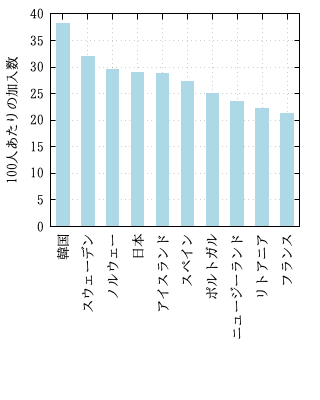
\includegraphics{Latexpng.png}
    \caption{光ファイバー回線の加入者数(100人あたり)}
    \label{fiber}
\end{figure}

% 本文(1)
% ーーー
% 節見出し(2)
\section{デジタル競争力ランキング}

% 本文(2)
国際経営開発研究所(IMD)の調査\cite{imd}によると、
日本のデジタル競争力のランキングは表\ref{degirank}に示すように、
調査対象の64カ国中、総合で28位、
準備分野で27位となっている。

% 表の挿入
% \begin{tabular}
% \end{tabular}    
% による表の記述を 
% \begin{table}[htbp]
% \end{table}
% で囲み
% \caption{}
% で表のタイトルを入れる.
% \label{}
% を使って表番号が参照できるようにする
% また,
% \centering
% で表が中央に来るようにする
\begin{table}[htbp]
    \centering
    \caption{デジタル競争力ランキング(64カ国中)}
    \label{degirank}
    \begin{tabular}{|c|c|c|}
        \hline
         国 & 総合 & 準備 \\
         \hline
         米国 & 1位 & 1位 \\
         \hline
         香港 & 2位 & 10位 \\
         \hline
         スウェーデン & 3位 & 6位 \\
         \hline
         デンマーク & 4位 & 2位 \\
         \hline
         シンガポール & 5位 & 11位 \\
        \hline
         韓国 & 12位 & 5位 \\
         \hline
         中国 & 15位 & 17位 \\
         \hline
         日本 & 28位 & 27位 \\
         \hline
     \end{tabular}
\end{table}

% ーーー
% 見出し(3)
\section{考察}
% 考察
%
% \begin{itemize}
% \end{itemize}
% を使って箇条書きで記述する
\begin{itemize}
    \item 日本のブロードバンド整備
    \begin{itemize}
        \item 世界第4位であり、早いスピードで幅広い範囲の検索が可能。
        \item インターネットの活用は日常生活に浸透しているといえる。
    \end{itemize}
\end{itemize}
\begin{itemize}
    \item 日本のデジタル競争力
    \begin{itemize}
        \item 日本のデジタル競争力のランキングは64ヵ国中28位である。
        \item 日本のブロードバンド整備を見ると競争力上位の国よりはかなり低い。
        
         
    \end{itemize}
\end{itemize}

% ここに参考文献が入る
%
\bibliographystyle{junsrt}
\bibliography{exercise.bib}

\end{document}